\section{Context and Motivation}
Data-driven decision-making is changing how we live and work. For every aspect of data science, machine learning, and advanced analytics, data scientists require data to help make decisions \cite{forEnterprises}. Big Tech companies like Google and Facebook to medium financial services organizations and insurance companies have always been data-driven. Big Data and Data Science are permeating all aspects of our lives. 

The concept of a Data Lake was driven by particular challenges that organizations were facing with the way data was handled, processed, and stored. Initially, what we used to is a data puddle, which is a single-purpose or single-project, started maintaining vast amounts of data themselves with almost no reuse in other applications in the same organization—these created information silos across various platforms. A demand was felt to have Data Lakes, which could solve data governance, data ownership, and data accessibility. A data lake could store any form of data, data as-is, data have no fixed schema,... so it could be analyzed and kept ready for consumption by consumer applications. 

Many researchers at the University of Science and Technology of Hanoi (USTH) and the Vietnam Academy of Science and Technology (VAST) work with data regularly. Suppose a dataset is frequently researched by multiple researchers from various departments and periods. However, data is currently arranged manually, even on the laboratory's storage, leading to duplication and difficult data discovery.

In this project, we attempt to develop a Data Lake to solve those challenges.

To start, we will use the C4 model to describe the software architecture because this application belongs to a more extensive system of ComLake, developed by a group of the software development team, supervised by Professor Tran Giang Son. 

\begin{figure}[H]
    \centering
    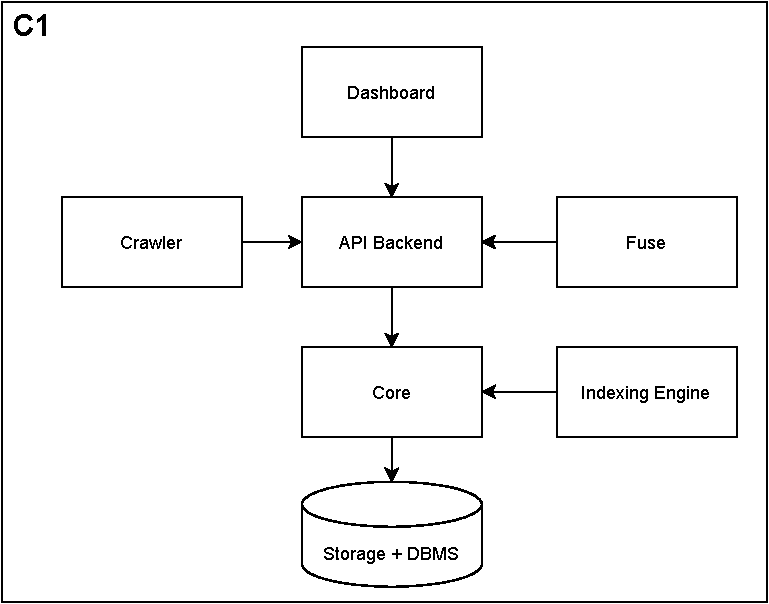
\includegraphics[width=1.0\textwidth, page={1}]{images/ComLake_arch.pdf}
    \caption{Level 1: System Context diagram: ComLake Overall Architecture diagram}
    \label{fig:C1}
\end{figure}
This is the System Context diagram for the ComLake system. The system comprises seven containers: a web application Dashboard, a server-side API Application, a data web Crawler, a Filesystem in USErspace (FUSE), an Image Indexing Engine using Machine Learning, a Core service that encapsulates distributed file system (DFS), and a database management system (DBMS).

The Dashboard, a ReactJS application that runs in the customer's web browser, will be the end-first user's point of contact. The Public API (API Backend in the figure) would handle authentication and authorization for external users and most internal services before being modified and given to the core API.

We will strive to build the Public API and Dashboard container. 

\section{Thesis Structure}
The thesis is divided into six main chapters to explain the development of Data Lake APIs and Dashboard.
\begin{itemize}
    \item The first chapter, Introduction, will discuss the fascinating subject of Data Lake APIs and Dashboards and the proposed solution in Chapter 1: Introduction.
    \item The second chapter, Objectives, we shall establish the project's standard requirements, present a quick summary of the system's operation, and present the reasons for its development.
    \item The third chapter, Requirement Analysis, will continue with the system's scenarios, use cases, object models, and dynamic models.
    \item The fourth chapter, Methodology, includes the entire functional specification and navigational paths that reflect the screen sequence. We will go through all of the tools and techniques utilized in the project, why they were chosen, and how the use cases were implemented in detail.
    \item The fifth chapter, Result and Discussion, we shall detail all of the functionalities that are implemented in the system
    \item The sixth chapter, Conclusions, provides conclusions about the project outcome and discusses the difficulties that exist during project development.
\end{itemize}
